\documentclass[1p]{elsarticle_modified}
%\bibliographystyle{elsarticle-num}

%\usepackage[colorlinks]{hyperref}
%\usepackage{abbrmath_seonhwa} %\Abb, \Ascr, \Acal ,\Abf, \Afrak
\usepackage{amsfonts}
\usepackage{amssymb}
\usepackage{amsmath}
\usepackage{amsthm}
\usepackage{scalefnt}
\usepackage{amsbsy}
\usepackage{kotex}
\usepackage{caption}
\usepackage{subfig}
\usepackage{color}
\usepackage{graphicx}
\usepackage{xcolor} %% white, black, red, green, blue, cyan, magenta, yellow
\usepackage{float}
\usepackage{setspace}
\usepackage{hyperref}

\usepackage{tikz}
\usetikzlibrary{arrows}

\usepackage{multirow}
\usepackage{array} % fixed length table
\usepackage{hhline}

%%%%%%%%%%%%%%%%%%%%%
\makeatletter
\renewcommand*\env@matrix[1][\arraystretch]{%
	\edef\arraystretch{#1}%
	\hskip -\arraycolsep
	\let\@ifnextchar\new@ifnextchar
	\array{*\c@MaxMatrixCols c}}
\makeatother %https://tex.stackexchange.com/questions/14071/how-can-i-increase-the-line-spacing-in-a-matrix
%%%%%%%%%%%%%%%

\usepackage[normalem]{ulem}

\newcommand{\msout}[1]{\ifmmode\text{\sout{\ensuremath{#1}}}\else\sout{#1}\fi}
%SOURCE: \msout is \stkout macro in https://tex.stackexchange.com/questions/20609/strikeout-in-math-mode

\newcommand{\cancel}[1]{
	\ifmmode
	{\color{red}\msout{#1}}
	\else
	{\color{red}\sout{#1}}
	\fi
}

\newcommand{\add}[1]{
	{\color{blue}\uwave{#1}}
}

\newcommand{\replace}[2]{
	\ifmmode
	{\color{red}\msout{#1}}{\color{blue}\uwave{#2}}
	\else
	{\color{red}\sout{#1}}{\color{blue}\uwave{#2}}
	\fi
}

\newcommand{\Sol}{\mathcal{S}} %segment
\newcommand{\D}{D} %diagram
\newcommand{\A}{\mathcal{A}} %arc


%%%%%%%%%%%%%%%%%%%%%%%%%%%%%5 test

\def\sl{\operatorname{\textup{SL}}(2,\Cbb)}
\def\psl{\operatorname{\textup{PSL}}(2,\Cbb)}
\def\quan{\mkern 1mu \triangleright \mkern 1mu}

\theoremstyle{definition}
\newtheorem{thm}{Theorem}[section]
\newtheorem{prop}[thm]{Proposition}
\newtheorem{lem}[thm]{Lemma}
\newtheorem{ques}[thm]{Question}
\newtheorem{cor}[thm]{Corollary}
\newtheorem{defn}[thm]{Definition}
\newtheorem{exam}[thm]{Example}
\newtheorem{rmk}[thm]{Remark}
\newtheorem{alg}[thm]{Algorithm}

\newcommand{\I}{\sqrt{-1}}
\begin{document}

%\begin{frontmatter}
%
%\title{Boundary parabolic representations of knots up to 8 crossings}
%
%%% Group authors per affiliation:
%\author{Yunhi Cho} 
%\address{Department of Mathematics, University of Seoul, Seoul, Korea}
%\ead{yhcho@uos.ac.kr}
%
%
%\author{Seonhwa Kim} %\fnref{s_kim}}
%\address{Center for Geometry and Physics, Institute for Basic Science, Pohang, 37673, Korea}
%\ead{ryeona17@ibs.re.kr}
%
%\author{Hyuk Kim}
%\address{Department of Mathematical Sciences, Seoul National University, Seoul 08826, Korea}
%\ead{hyukkim@snu.ac.kr}
%
%\author{Seokbeom Yoon}
%\address{Department of Mathematical Sciences, Seoul National University, Seoul, 08826,  Korea}
%\ead{sbyoon15@snu.ac.kr}
%
%\begin{abstract}
%We find all boundary parabolic representation of knots up to 8 crossings.
%
%\end{abstract}
%\begin{keyword}
%    \MSC[2010] 57M25 
%\end{keyword}
%
%\end{frontmatter}

%\linenumbers
%\tableofcontents
%
\newcommand\colored[1]{\textcolor{white}{\rule[-0.35ex]{0.8em}{1.4ex}}\kern-0.8em\color{red} #1}%
%\newcommand\colored[1]{\textcolor{white}{ #1}\kern-2.17ex	\textcolor{white}{ #1}\kern-1.81ex	\textcolor{white}{ #1}\kern-2.15ex\color{red}#1	}

{\Large $\underline{12a_{0084}~(K12a_{0084})}$}

\setlength{\tabcolsep}{10pt}
\renewcommand{\arraystretch}{1.6}
\vspace{1cm}\begin{tabular}{m{100pt}>{\centering\arraybackslash}m{274pt}}
\multirow{5}{120pt}{
	\centering
	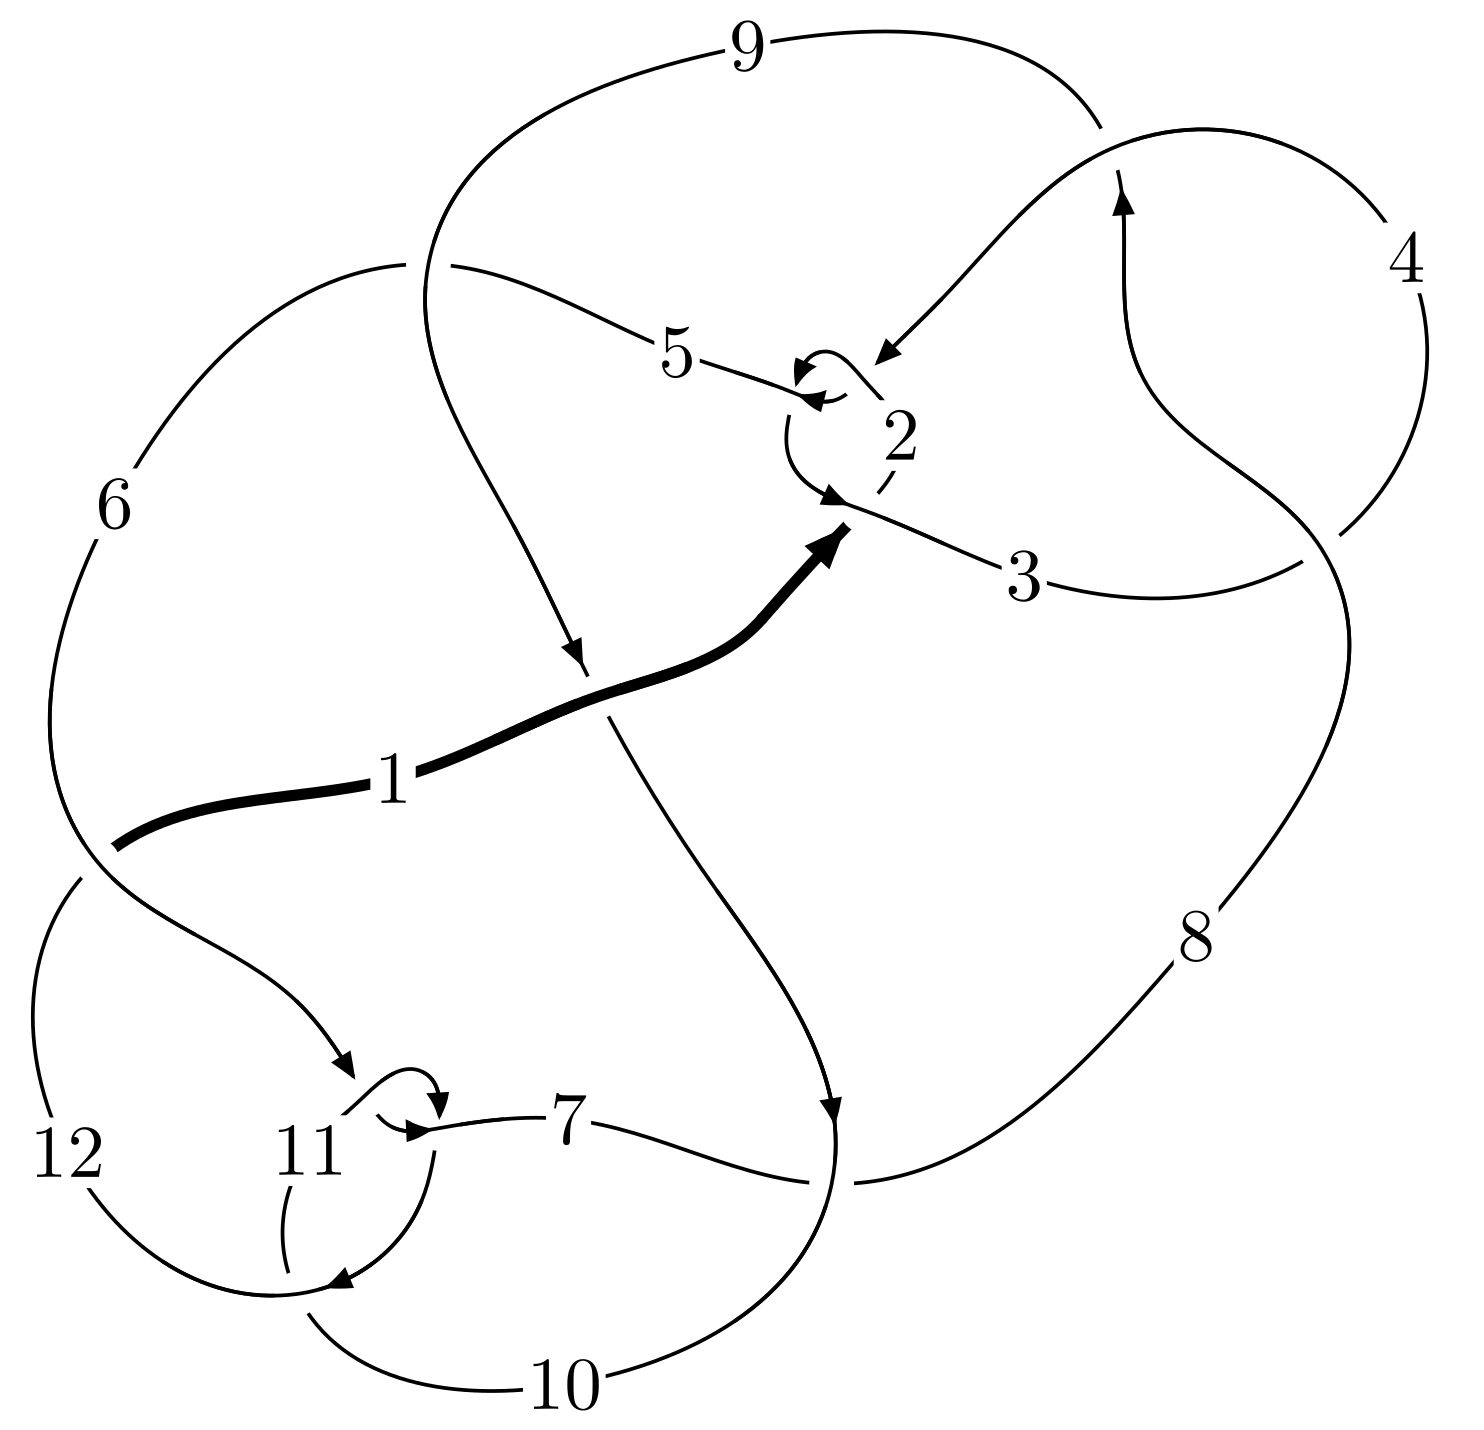
\includegraphics[width=112pt]{../../../GIT/diagram.site/Diagrams/png/885_12a_0084.png}\\
\ \ \ A knot diagram\footnotemark}&
\allowdisplaybreaks
\textbf{Linearized knot diagam} \\
\cline{2-2}
 &
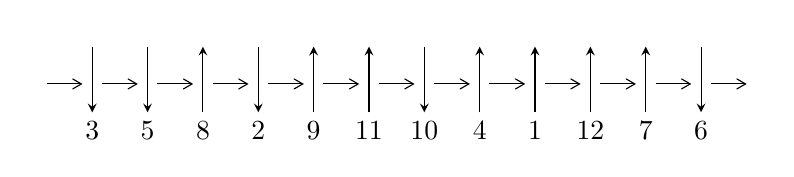
\begin{tikzpicture}[x=20pt, y=17pt]
	% nodes
	\node (C0) at (0, 0) {};
	\node (C1) at (1, 0) {};
	\node (C1U) at (1, +1) {};
	\node (C1D) at (1, -1) {3};

	\node (C2) at (2, 0) {};
	\node (C2U) at (2, +1) {};
	\node (C2D) at (2, -1) {5};

	\node (C3) at (3, 0) {};
	\node (C3U) at (3, +1) {};
	\node (C3D) at (3, -1) {8};

	\node (C4) at (4, 0) {};
	\node (C4U) at (4, +1) {};
	\node (C4D) at (4, -1) {2};

	\node (C5) at (5, 0) {};
	\node (C5U) at (5, +1) {};
	\node (C5D) at (5, -1) {9};

	\node (C6) at (6, 0) {};
	\node (C6U) at (6, +1) {};
	\node (C6D) at (6, -1) {11};

	\node (C7) at (7, 0) {};
	\node (C7U) at (7, +1) {};
	\node (C7D) at (7, -1) {10};

	\node (C8) at (8, 0) {};
	\node (C8U) at (8, +1) {};
	\node (C8D) at (8, -1) {4};

	\node (C9) at (9, 0) {};
	\node (C9U) at (9, +1) {};
	\node (C9D) at (9, -1) {1};

	\node (C10) at (10, 0) {};
	\node (C10U) at (10, +1) {};
	\node (C10D) at (10, -1) {12};

	\node (C11) at (11, 0) {};
	\node (C11U) at (11, +1) {};
	\node (C11D) at (11, -1) {7};

	\node (C12) at (12, 0) {};
	\node (C12U) at (12, +1) {};
	\node (C12D) at (12, -1) {6};
	\node (C13) at (13, 0) {};

	% arrows
	\draw[->,>={angle 60}]
	(C0) edge (C1) (C1) edge (C2) (C2) edge (C3) (C3) edge (C4) (C4) edge (C5) (C5) edge (C6) (C6) edge (C7) (C7) edge (C8) (C8) edge (C9) (C9) edge (C10) (C10) edge (C11) (C11) edge (C12) (C12) edge (C13) ;	\draw[->,>=stealth]
	(C1U) edge (C1D) (C2U) edge (C2D) (C3D) edge (C3U) (C4U) edge (C4D) (C5D) edge (C5U) (C6D) edge (C6U) (C7U) edge (C7D) (C8D) edge (C8U) (C9D) edge (C9U) (C10D) edge (C10U) (C11D) edge (C11U) (C12U) edge (C12D) ;
	\end{tikzpicture} \\
\hhline{~~} \\& 
\textbf{Solving Sequence} \\ \cline{2-2} 
 &
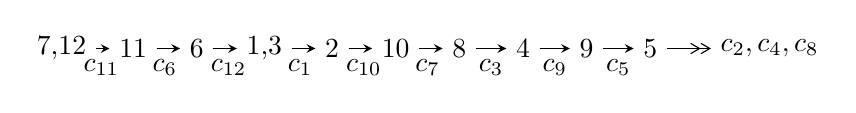
\begin{tikzpicture}[x=23pt, y=7pt]
	% node
	\node (A0) at (-1/8, 0) {7,12};
	\node (A1) at (1, 0) {11};
	\node (A2) at (2, 0) {6};
	\node (A3) at (49/16, 0) {1,3};
	\node (A4) at (33/8, 0) {2};
	\node (A5) at (41/8, 0) {10};
	\node (A6) at (49/8, 0) {8};
	\node (A7) at (57/8, 0) {4};
	\node (A8) at (65/8, 0) {9};
	\node (A9) at (73/8, 0) {5};
	\node (C1) at (1/2, -1) {$c_{11}$};
	\node (C2) at (3/2, -1) {$c_{6}$};
	\node (C3) at (5/2, -1) {$c_{12}$};
	\node (C4) at (29/8, -1) {$c_{1}$};
	\node (C5) at (37/8, -1) {$c_{10}$};
	\node (C6) at (45/8, -1) {$c_{7}$};
	\node (C7) at (53/8, -1) {$c_{3}$};
	\node (C8) at (61/8, -1) {$c_{9}$};
	\node (C9) at (69/8, -1) {$c_{5}$};
	\node (A10) at (11, 0) {$c_{2},c_{4},c_{8}$};

	% edge
	\draw[->,>=stealth]	
	(A0) edge (A1) (A1) edge (A2) (A2) edge (A3) (A3) edge (A4) (A4) edge (A5) (A5) edge (A6) (A6) edge (A7) (A7) edge (A8) (A8) edge (A9) ;
	\draw[->>,>={angle 60}]	
	(A9) edge (A10);
\end{tikzpicture} \\ 

\end{tabular} \\

\footnotetext{
The image of knot diagram is generated by the software ``\textbf{Draw programme}" developed by Andrew Bartholomew(\url{http://www.layer8.co.uk/maths/draw/index.htm\#Running-draw}), where we modified some parts for our purpose(\url{https://github.com/CATsTAILs/LinksPainter}).
}\phantom \\ \newline 
\centering \textbf{Ideals for irreducible components\footnotemark of $X_{\text{par}}$} 
 
\begin{align*}
I^u_{1}&=\langle 
- u^{107}+u^{106}+\cdots+b+u,\;3 u^{107}-3 u^{106}+\cdots+a+1,\;u^{108}-2 u^{107}+\cdots+3 u-1\rangle \\
I^u_{2}&=\langle 
u^3+b- u-1,\;- u^7+2 u^5+u^4-2 u^3- u^2+a+1,\;u^9+u^8-2 u^7-3 u^6+u^5+3 u^4+2 u^3- u-1\rangle \\
\\
\end{align*}
\raggedright * 2 irreducible components of $\dim_{\mathbb{C}}=0$, with total 117 representations.\\
\footnotetext{All coefficients of polynomials are rational numbers. But the coefficients are sometimes approximated in decimal forms when there is not enough margin.}
\newpage
\renewcommand{\arraystretch}{1}
\centering \section*{I. $I^u_{1}= \langle - u^{107}+u^{106}+\cdots+b+u,\;3 u^{107}-3 u^{106}+\cdots+a+1,\;u^{108}-2 u^{107}+\cdots+3 u-1 \rangle$}
\flushleft \textbf{(i) Arc colorings}\\
\begin{tabular}{m{7pt} m{180pt} m{7pt} m{180pt} }
\flushright $a_{7}=$&$\begin{pmatrix}0\\u\end{pmatrix}$ \\
\flushright $a_{12}=$&$\begin{pmatrix}1\\0\end{pmatrix}$ \\
\flushright $a_{11}=$&$\begin{pmatrix}1\\u^2\end{pmatrix}$ \\
\flushright $a_{6}=$&$\begin{pmatrix}- u\\- u^3+u\end{pmatrix}$ \\
\flushright $a_{1}=$&$\begin{pmatrix}u^4- u^2+1\\u^6-2 u^4+u^2\end{pmatrix}$ \\
\flushright $a_{3}=$&$\begin{pmatrix}-3 u^{107}+3 u^{106}+\cdots+4 u-1\\u^{107}- u^{106}+\cdots+3 u^2- u\end{pmatrix}$ \\
\flushright $a_{2}=$&$\begin{pmatrix}2 u^{107}-2 u^{106}+\cdots-3 u+1\\- u^{107}+u^{106}+\cdots-2 u^2+u\end{pmatrix}$ \\
\flushright $a_{10}=$&$\begin{pmatrix}- u^2+1\\u^2\end{pmatrix}$ \\
\flushright $a_{8}=$&$\begin{pmatrix}- u^5+2 u^3- u\\u^5- u^3+u\end{pmatrix}$ \\
\flushright $a_{4}=$&$\begin{pmatrix}- u^{107}+u^{106}+\cdots+3 u^3-3 u^2\\u^{107}- u^{106}+\cdots-4 u^4+u^2\end{pmatrix}$ \\
\flushright $a_{9}=$&$\begin{pmatrix}- u^{12}+3 u^{10}-5 u^8+4 u^6-2 u^4- u^2+1\\- u^{14}+4 u^{12}-7 u^{10}+6 u^8-2 u^6+u^2\end{pmatrix}$ \\
\flushright $a_{5}=$&$\begin{pmatrix}u^{23}-6 u^{21}+\cdots+2 u^3-2 u\\u^{25}-7 u^{23}+\cdots-2 u^3+u\end{pmatrix}$\\&\end{tabular}
\flushleft \textbf{(ii) Obstruction class $= -1$}\\~\\
\flushleft \textbf{(iii) Cusp Shapes $= 14 u^{107}-15 u^{106}+\cdots-29 u+15$}\\~\\
\newpage\renewcommand{\arraystretch}{1}
\flushleft \textbf{(iv) u-Polynomials at the component}\newline \\
\begin{tabular}{m{50pt}|m{274pt}}
Crossings & \hspace{64pt}u-Polynomials at each crossing \\
\hline $$\begin{aligned}c_{1}\end{aligned}$$&$\begin{aligned}
&u^{108}+50 u^{107}+\cdots+43 u+1
\end{aligned}$\\
\hline $$\begin{aligned}c_{2},c_{4}\end{aligned}$$&$\begin{aligned}
&u^{108}-10 u^{107}+\cdots+11 u-1
\end{aligned}$\\
\hline $$\begin{aligned}c_{3},c_{8}\end{aligned}$$&$\begin{aligned}
&u^{108}+u^{107}+\cdots-7424 u^2+512
\end{aligned}$\\
\hline $$\begin{aligned}c_{5}\end{aligned}$$&$\begin{aligned}
&u^{108}-2 u^{107}+\cdots+2153835 u-699025
\end{aligned}$\\
\hline $$\begin{aligned}c_{6},c_{11}\end{aligned}$$&$\begin{aligned}
&u^{108}-2 u^{107}+\cdots+3 u-1
\end{aligned}$\\
\hline $$\begin{aligned}c_{7},c_{12}\end{aligned}$$&$\begin{aligned}
&u^{108}-6 u^{107}+\cdots+11 u-1
\end{aligned}$\\
\hline $$\begin{aligned}c_{9}\end{aligned}$$&$\begin{aligned}
&u^{108}+14 u^{107}+\cdots+4453 u+349
\end{aligned}$\\
\hline $$\begin{aligned}c_{10}\end{aligned}$$&$\begin{aligned}
&u^{108}-58 u^{107}+\cdots+u+1
\end{aligned}$\\
\hline
\end{tabular}\\~\\
\newpage\renewcommand{\arraystretch}{1}
\flushleft \textbf{(v) Riley Polynomials at the component}\newline \\
\begin{tabular}{m{50pt}|m{274pt}}
Crossings & \hspace{64pt}Riley Polynomials at each crossing \\
\hline $$\begin{aligned}c_{1}\end{aligned}$$&$\begin{aligned}
&y^{108}+26 y^{107}+\cdots-1883 y+1
\end{aligned}$\\
\hline $$\begin{aligned}c_{2},c_{4}\end{aligned}$$&$\begin{aligned}
&y^{108}-50 y^{107}+\cdots-43 y+1
\end{aligned}$\\
\hline $$\begin{aligned}c_{3},c_{8}\end{aligned}$$&$\begin{aligned}
&y^{108}-57 y^{107}+\cdots-7602176 y+262144
\end{aligned}$\\
\hline $$\begin{aligned}c_{5}\end{aligned}$$&$\begin{aligned}
&y^{108}-42 y^{107}+\cdots-6625342064775 y+488635950625
\end{aligned}$\\
\hline $$\begin{aligned}c_{6},c_{11}\end{aligned}$$&$\begin{aligned}
&y^{108}-58 y^{107}+\cdots+y+1
\end{aligned}$\\
\hline $$\begin{aligned}c_{7},c_{12}\end{aligned}$$&$\begin{aligned}
&y^{108}+86 y^{107}+\cdots+121 y+1
\end{aligned}$\\
\hline $$\begin{aligned}c_{9}\end{aligned}$$&$\begin{aligned}
&y^{108}-6 y^{107}+\cdots-1457151 y+121801
\end{aligned}$\\
\hline $$\begin{aligned}c_{10}\end{aligned}$$&$\begin{aligned}
&y^{108}-14 y^{107}+\cdots-7 y+1
\end{aligned}$\\
\hline
\end{tabular}\\~\\
\newpage\flushleft \textbf{(vi) Complex Volumes and Cusp Shapes}
$$\begin{array}{c|c|c}  
\text{Solutions to }I^u_{1}& \I (\text{vol} + \sqrt{-1}CS) & \text{Cusp shape}\\
 \hline 
\begin{aligned}
u &= \phantom{-}0.996236 + 0.045280 I \\
a &= -0.116744 + 1.006360 I \\
b &= -0.406874 + 0.889939 I\end{aligned}
 & \phantom{-}1.66851 + 2.03339 I & \phantom{-0.000000 } 0 \\ \hline\begin{aligned}
u &= \phantom{-}0.996236 - 0.045280 I \\
a &= -0.116744 - 1.006360 I \\
b &= -0.406874 - 0.889939 I\end{aligned}
 & \phantom{-}1.66851 - 2.03339 I & \phantom{-0.000000 } 0 \\ \hline\begin{aligned}
u &= -0.862530 + 0.521960 I \\
a &= \phantom{-}1.133140 + 0.012092 I \\
b &= \phantom{-}0.830795 - 0.379581 I\end{aligned}
 & -2.08646 - 5.96170 I & \phantom{-0.000000 } 0 \\ \hline\begin{aligned}
u &= -0.862530 - 0.521960 I \\
a &= \phantom{-}1.133140 - 0.012092 I \\
b &= \phantom{-}0.830795 + 0.379581 I\end{aligned}
 & -2.08646 + 5.96170 I & \phantom{-0.000000 } 0 \\ \hline\begin{aligned}
u &= \phantom{-}0.844591 + 0.507051 I \\
a &= \phantom{-}0.59353 + 1.36298 I \\
b &= \phantom{-}0.270864 - 0.952687 I\end{aligned}
 & -2.96700 + 3.56740 I & \phantom{-0.000000 } 0 \\ \hline\begin{aligned}
u &= \phantom{-}0.844591 - 0.507051 I \\
a &= \phantom{-}0.59353 - 1.36298 I \\
b &= \phantom{-}0.270864 + 0.952687 I\end{aligned}
 & -2.96700 - 3.56740 I & \phantom{-0.000000 } 0 \\ \hline\begin{aligned}
u &= -0.794168 + 0.557145 I \\
a &= \phantom{-}0.266509 - 0.777339 I \\
b &= \phantom{-}0.464499 - 0.344043 I\end{aligned}
 & -2.97176 - 0.64254 I & \phantom{-0.000000 } 0 \\ \hline\begin{aligned}
u &= -0.794168 - 0.557145 I \\
a &= \phantom{-}0.266509 + 0.777339 I \\
b &= \phantom{-}0.464499 + 0.344043 I\end{aligned}
 & -2.97176 + 0.64254 I & \phantom{-0.000000 } 0 \\ \hline\begin{aligned}
u &= \phantom{-}0.885383 + 0.534389 I \\
a &= -0.603383 - 0.155335 I \\
b &= -0.367723 + 0.938689 I\end{aligned}
 & \phantom{-}2.59244 + 6.40382 I & \phantom{-0.000000 } 0 \\ \hline\begin{aligned}
u &= \phantom{-}0.885383 - 0.534389 I \\
a &= -0.603383 + 0.155335 I \\
b &= -0.367723 - 0.938689 I\end{aligned}
 & \phantom{-}2.59244 - 6.40382 I & \phantom{-0.000000 } 0\\
 \hline 
 \end{array}$$\newpage$$\begin{array}{c|c|c}  
\text{Solutions to }I^u_{1}& \I (\text{vol} + \sqrt{-1}CS) & \text{Cusp shape}\\
 \hline 
\begin{aligned}
u &= \phantom{-}0.876654 + 0.553713 I \\
a &= \phantom{-}1.138340 - 0.046475 I \\
b &= \phantom{-}0.354844 - 0.826320 I\end{aligned}
 & \phantom{-}0.41046 + 11.93020 I & \phantom{-0.000000 } 0 \\ \hline\begin{aligned}
u &= \phantom{-}0.876654 - 0.553713 I \\
a &= \phantom{-}1.138340 + 0.046475 I \\
b &= \phantom{-}0.354844 + 0.826320 I\end{aligned}
 & \phantom{-}0.41046 - 11.93020 I & \phantom{-0.000000 } 0 \\ \hline\begin{aligned}
u &= -0.956750\phantom{ +0.000000I} \\
a &= \phantom{-}0.894676\phantom{ +0.000000I} \\
b &= -1.61493\phantom{ +0.000000I}\end{aligned}
 & \phantom{-}0.334264\phantom{ +0.000000I} & \phantom{-0.000000 } 0 \\ \hline\begin{aligned}
u &= -0.839356 + 0.456799 I \\
a &= -0.506274 - 0.352044 I \\
b &= -0.973741 - 0.147203 I\end{aligned}
 & -0.86996 - 1.97916 I & \phantom{-0.000000 } 0 \\ \hline\begin{aligned}
u &= -0.839356 - 0.456799 I \\
a &= -0.506274 + 0.352044 I \\
b &= -0.973741 + 0.147203 I\end{aligned}
 & -0.86996 + 1.97916 I & \phantom{-0.000000 } 0 \\ \hline\begin{aligned}
u &= -1.048940 + 0.048886 I \\
a &= -1.133180 + 0.113072 I \\
b &= \phantom{-}0.343147 + 0.845942 I\end{aligned}
 & \phantom{-}6.58179 - 1.97370 I & \phantom{-0.000000 } 0 \\ \hline\begin{aligned}
u &= -1.048940 - 0.048886 I \\
a &= -1.133180 - 0.113072 I \\
b &= \phantom{-}0.343147 - 0.845942 I\end{aligned}
 & \phantom{-}6.58179 + 1.97370 I & \phantom{-0.000000 } 0 \\ \hline\begin{aligned}
u &= \phantom{-}0.948392 + 0.456770 I \\
a &= \phantom{-}0.858154 - 0.677501 I \\
b &= \phantom{-}0.030428 + 1.311010 I\end{aligned}
 & \phantom{-}3.81145 + 3.11422 I & \phantom{-0.000000 } 0 \\ \hline\begin{aligned}
u &= \phantom{-}0.948392 - 0.456770 I \\
a &= \phantom{-}0.858154 + 0.677501 I \\
b &= \phantom{-}0.030428 - 1.311010 I\end{aligned}
 & \phantom{-}3.81145 - 3.11422 I & \phantom{-0.000000 } 0 \\ \hline\begin{aligned}
u &= -1.058660 + 0.084126 I \\
a &= \phantom{-}1.191570 - 0.207622 I \\
b &= -0.44160 - 1.44697 I\end{aligned}
 & \phantom{-}4.80577 - 7.59628 I & \phantom{-0.000000 } 0\\
 \hline 
 \end{array}$$\newpage$$\begin{array}{c|c|c}  
\text{Solutions to }I^u_{1}& \I (\text{vol} + \sqrt{-1}CS) & \text{Cusp shape}\\
 \hline 
\begin{aligned}
u &= -1.058660 - 0.084126 I \\
a &= \phantom{-}1.191570 + 0.207622 I \\
b &= -0.44160 + 1.44697 I\end{aligned}
 & \phantom{-}4.80577 + 7.59628 I & \phantom{-0.000000 } 0 \\ \hline\begin{aligned}
u &= -0.736275 + 0.560642 I \\
a &= \phantom{-}0.509790 + 0.501835 I \\
b &= -0.391752 + 0.666181 I\end{aligned}
 & -3.13683 - 3.82711 I & \phantom{-0.000000 } 0 \\ \hline\begin{aligned}
u &= -0.736275 - 0.560642 I \\
a &= \phantom{-}0.509790 - 0.501835 I \\
b &= -0.391752 - 0.666181 I\end{aligned}
 & -3.13683 + 3.82711 I & \phantom{-0.000000 } 0 \\ \hline\begin{aligned}
u &= \phantom{-}1.051040 + 0.322763 I \\
a &= -0.87818 + 1.25855 I \\
b &= -1.10882 - 1.15799 I\end{aligned}
 & \phantom{-}2.55355 - 1.82439 I & \phantom{-0.000000 } 0 \\ \hline\begin{aligned}
u &= \phantom{-}1.051040 - 0.322763 I \\
a &= -0.87818 - 1.25855 I \\
b &= -1.10882 + 1.15799 I\end{aligned}
 & \phantom{-}2.55355 + 1.82439 I & \phantom{-0.000000 } 0 \\ \hline\begin{aligned}
u &= -0.743951 + 0.441122 I \\
a &= -0.168733 - 0.150783 I \\
b &= -0.556383 - 0.687073 I\end{aligned}
 & -1.16073 - 1.79746 I & \phantom{-0.000000 -}0. + 5.56509 I \\ \hline\begin{aligned}
u &= -0.743951 - 0.441122 I \\
a &= -0.168733 + 0.150783 I \\
b &= -0.556383 + 0.687073 I\end{aligned}
 & -1.16073 + 1.79746 I & \phantom{-0.000000 } 0. - 5.56509 I \\ \hline\begin{aligned}
u &= \phantom{-}1.048310 + 0.450986 I \\
a &= -1.40818 + 1.29023 I \\
b &= -0.72561 - 1.90324 I\end{aligned}
 & \phantom{-}2.48243 - 1.91335 I & \phantom{-0.000000 } 0 \\ \hline\begin{aligned}
u &= \phantom{-}1.048310 - 0.450986 I \\
a &= -1.40818 - 1.29023 I \\
b &= -0.72561 + 1.90324 I\end{aligned}
 & \phantom{-}2.48243 + 1.91335 I & \phantom{-0.000000 } 0 \\ \hline\begin{aligned}
u &= \phantom{-}0.624825 + 0.574772 I \\
a &= \phantom{-}1.028940 + 0.598373 I \\
b &= \phantom{-}0.699771 - 0.402827 I\end{aligned}
 & -0.29917 - 7.43550 I & -0.31843 + 4.49348 I\\
 \hline 
 \end{array}$$\newpage$$\begin{array}{c|c|c}  
\text{Solutions to }I^u_{1}& \I (\text{vol} + \sqrt{-1}CS) & \text{Cusp shape}\\
 \hline 
\begin{aligned}
u &= \phantom{-}0.624825 - 0.574772 I \\
a &= \phantom{-}1.028940 - 0.598373 I \\
b &= \phantom{-}0.699771 + 0.402827 I\end{aligned}
 & -0.29917 + 7.43550 I & -0.31843 - 4.49348 I \\ \hline\begin{aligned}
u &= \phantom{-}0.677012 + 0.490046 I \\
a &= \phantom{-}1.91943 - 0.37048 I \\
b &= \phantom{-}0.010605 - 0.151479 I\end{aligned}
 & -3.45158 + 0.56668 I & -1.98152 + 0.95502 I \\ \hline\begin{aligned}
u &= \phantom{-}0.677012 - 0.490046 I \\
a &= \phantom{-}1.91943 + 0.37048 I \\
b &= \phantom{-}0.010605 + 0.151479 I\end{aligned}
 & -3.45158 - 0.56668 I & -1.98152 - 0.95502 I \\ \hline\begin{aligned}
u &= \phantom{-}0.143847 + 0.816906 I \\
a &= \phantom{-}3.60584 - 1.75236 I \\
b &= -2.72020 + 1.87600 I\end{aligned}
 & \phantom{-}3.99543 - 12.45750 I & \phantom{-}3.16743 + 7.87882 I \\ \hline\begin{aligned}
u &= \phantom{-}0.143847 - 0.816906 I \\
a &= \phantom{-}3.60584 + 1.75236 I \\
b &= -2.72020 - 1.87600 I\end{aligned}
 & \phantom{-}3.99543 + 12.45750 I & \phantom{-}3.16743 - 7.87882 I \\ \hline\begin{aligned}
u &= \phantom{-}0.131097 + 0.814628 I \\
a &= -2.82764 + 1.44556 I \\
b &= \phantom{-}2.19358 - 1.64273 I\end{aligned}
 & \phantom{-}6.19290 - 6.68872 I & \phantom{-}6.18602 + 3.85805 I \\ \hline\begin{aligned}
u &= \phantom{-}0.131097 - 0.814628 I \\
a &= -2.82764 - 1.44556 I \\
b &= \phantom{-}2.19358 + 1.64273 I\end{aligned}
 & \phantom{-}6.19290 + 6.68872 I & \phantom{-}6.18602 - 3.85805 I \\ \hline\begin{aligned}
u &= -0.638302 + 0.513402 I \\
a &= \phantom{-}0.298195 - 0.327642 I \\
b &= \phantom{-}0.150510 + 1.281760 I\end{aligned}
 & -2.71730 + 1.71656 I & -2.69239 - 1.49770 I \\ \hline\begin{aligned}
u &= -0.638302 - 0.513402 I \\
a &= \phantom{-}0.298195 + 0.327642 I \\
b &= \phantom{-}0.150510 - 1.281760 I\end{aligned}
 & -2.71730 - 1.71656 I & -2.69239 + 1.49770 I \\ \hline\begin{aligned}
u &= \phantom{-}0.084734 + 0.810618 I \\
a &= -0.281035 + 0.148733 I \\
b &= \phantom{-}0.451303 - 0.663859 I\end{aligned}
 & \phantom{-}7.50477 - 2.37218 I & \phantom{-}7.60940 + 2.45508 I\\
 \hline 
 \end{array}$$\newpage$$\begin{array}{c|c|c}  
\text{Solutions to }I^u_{1}& \I (\text{vol} + \sqrt{-1}CS) & \text{Cusp shape}\\
 \hline 
\begin{aligned}
u &= \phantom{-}0.084734 - 0.810618 I \\
a &= -0.281035 - 0.148733 I \\
b &= \phantom{-}0.451303 + 0.663859 I\end{aligned}
 & \phantom{-}7.50477 + 2.37218 I & \phantom{-}7.60940 - 2.45508 I \\ \hline\begin{aligned}
u &= \phantom{-}0.062002 + 0.809107 I \\
a &= -0.694063 + 0.273767 I \\
b &= \phantom{-}0.216786 + 0.332131 I\end{aligned}
 & \phantom{-}6.29498 + 3.41320 I & \phantom{-}6.03563 - 2.91284 I \\ \hline\begin{aligned}
u &= \phantom{-}0.062002 - 0.809107 I \\
a &= -0.694063 - 0.273767 I \\
b &= \phantom{-}0.216786 - 0.332131 I\end{aligned}
 & \phantom{-}6.29498 - 3.41320 I & \phantom{-}6.03563 + 2.91284 I \\ \hline\begin{aligned}
u &= \phantom{-}0.597470 + 0.547708 I \\
a &= -0.948340 - 0.065977 I \\
b &= -0.633409 + 0.082605 I\end{aligned}
 & \phantom{-}1.79154 - 2.04029 I & \phantom{-}2.75012 + 0.45973 I \\ \hline\begin{aligned}
u &= \phantom{-}0.597470 - 0.547708 I \\
a &= -0.948340 + 0.065977 I \\
b &= -0.633409 - 0.082605 I\end{aligned}
 & \phantom{-}1.79154 + 2.04029 I & \phantom{-}2.75012 - 0.45973 I \\ \hline\begin{aligned}
u &= -0.130219 + 0.799256 I \\
a &= \phantom{-}1.52061 + 2.52254 I \\
b &= -0.66932 - 1.91757 I\end{aligned}
 & \phantom{-}1.23189 + 6.19452 I & \phantom{-}2.03888 - 5.46938 I \\ \hline\begin{aligned}
u &= -0.130219 - 0.799256 I \\
a &= \phantom{-}1.52061 - 2.52254 I \\
b &= -0.66932 + 1.91757 I\end{aligned}
 & \phantom{-}1.23189 - 6.19452 I & \phantom{-}2.03888 + 5.46938 I \\ \hline\begin{aligned}
u &= \phantom{-}0.124021 + 0.786804 I \\
a &= \phantom{-}1.37622 - 2.82570 I \\
b &= -1.15779 + 2.57523 I\end{aligned}
 & \phantom{-}0.12959 - 3.69092 I & \phantom{-}3.30927 + 4.30775 I \\ \hline\begin{aligned}
u &= \phantom{-}0.124021 - 0.786804 I \\
a &= \phantom{-}1.37622 + 2.82570 I \\
b &= -1.15779 - 2.57523 I\end{aligned}
 & \phantom{-}0.12959 + 3.69092 I & \phantom{-}3.30927 - 4.30775 I \\ \hline\begin{aligned}
u &= -0.102979 + 0.784283 I \\
a &= -1.95071 - 1.53814 I \\
b &= \phantom{-}1.05096 + 1.30453 I\end{aligned}
 & \phantom{-}2.11051 + 1.68118 I & \phantom{-}3.82795 - 0.19790 I\\
 \hline 
 \end{array}$$\newpage$$\begin{array}{c|c|c}  
\text{Solutions to }I^u_{1}& \I (\text{vol} + \sqrt{-1}CS) & \text{Cusp shape}\\
 \hline 
\begin{aligned}
u &= -0.102979 - 0.784283 I \\
a &= -1.95071 + 1.53814 I \\
b &= \phantom{-}1.05096 - 1.30453 I\end{aligned}
 & \phantom{-}2.11051 - 1.68118 I & \phantom{-}3.82795 + 0.19790 I \\ \hline\begin{aligned}
u &= \phantom{-}1.162950 + 0.364150 I \\
a &= \phantom{-}1.036500 - 0.765772 I \\
b &= \phantom{-}0.37000 + 1.58101 I\end{aligned}
 & \phantom{-}3.58952 + 2.14988 I & \phantom{-0.000000 } 0 \\ \hline\begin{aligned}
u &= \phantom{-}1.162950 - 0.364150 I \\
a &= \phantom{-}1.036500 + 0.765772 I \\
b &= \phantom{-}0.37000 - 1.58101 I\end{aligned}
 & \phantom{-}3.58952 - 2.14988 I & \phantom{-0.000000 } 0 \\ \hline\begin{aligned}
u &= -0.178445 + 0.755692 I \\
a &= -0.96043 + 1.86608 I \\
b &= \phantom{-}0.99543 - 1.15166 I\end{aligned}
 & -0.33248 + 1.46092 I & \phantom{-}3.18525 + 1.98059 I \\ \hline\begin{aligned}
u &= -0.178445 - 0.755692 I \\
a &= -0.96043 - 1.86608 I \\
b &= \phantom{-}0.99543 + 1.15166 I\end{aligned}
 & -0.33248 - 1.46092 I & \phantom{-}3.18525 - 1.98059 I \\ \hline\begin{aligned}
u &= -1.136950 + 0.452088 I \\
a &= \phantom{-}0.02675 - 2.17145 I \\
b &= -3.00297 + 0.76343 I\end{aligned}
 & \phantom{-}0.82492 - 2.79638 I & \phantom{-0.000000 } 0 \\ \hline\begin{aligned}
u &= -1.136950 - 0.452088 I \\
a &= \phantom{-}0.02675 + 2.17145 I \\
b &= -3.00297 - 0.76343 I\end{aligned}
 & \phantom{-}0.82492 + 2.79638 I & \phantom{-0.000000 } 0 \\ \hline\begin{aligned}
u &= \phantom{-}1.155100 + 0.420420 I \\
a &= \phantom{-}0.09813 - 1.43768 I \\
b &= \phantom{-}1.40058 + 0.80355 I\end{aligned}
 & \phantom{-}4.17176 + 2.11595 I & \phantom{-0.000000 } 0 \\ \hline\begin{aligned}
u &= \phantom{-}1.155100 - 0.420420 I \\
a &= \phantom{-}0.09813 + 1.43768 I \\
b &= \phantom{-}1.40058 - 0.80355 I\end{aligned}
 & \phantom{-}4.17176 - 2.11595 I & \phantom{-0.000000 } 0 \\ \hline\begin{aligned}
u &= \phantom{-}1.145120 + 0.469099 I \\
a &= -0.19347 + 2.77467 I \\
b &= -2.56390 - 1.37308 I\end{aligned}
 & \phantom{-}0.67784 + 5.12770 I & \phantom{-0.000000 } 0\\
 \hline 
 \end{array}$$\newpage$$\begin{array}{c|c|c}  
\text{Solutions to }I^u_{1}& \I (\text{vol} + \sqrt{-1}CS) & \text{Cusp shape}\\
 \hline 
\begin{aligned}
u &= \phantom{-}1.145120 - 0.469099 I \\
a &= -0.19347 - 2.77467 I \\
b &= -2.56390 + 1.37308 I\end{aligned}
 & \phantom{-}0.67784 - 5.12770 I & \phantom{-0.000000 } 0 \\ \hline\begin{aligned}
u &= \phantom{-}0.757499\phantom{ +0.000000I} \\
a &= -0.645860\phantom{ +0.000000I} \\
b &= -0.119944\phantom{ +0.000000I}\end{aligned}
 & \phantom{-}1.00529\phantom{ +0.000000I} & \phantom{-}10.9620\phantom{ +0.000000I} \\ \hline\begin{aligned}
u &= -1.141430 + 0.505632 I \\
a &= \phantom{-}1.09724 - 1.94822 I \\
b &= -2.74030 - 0.37394 I\end{aligned}
 & \phantom{-}1.52022 - 9.42870 I & \phantom{-0.000000 } 0 \\ \hline\begin{aligned}
u &= -1.141430 - 0.505632 I \\
a &= \phantom{-}1.09724 + 1.94822 I \\
b &= -2.74030 + 0.37394 I\end{aligned}
 & \phantom{-}1.52022 + 9.42870 I & \phantom{-0.000000 } 0 \\ \hline\begin{aligned}
u &= -1.164500 + 0.479359 I \\
a &= -0.09977 + 1.55618 I \\
b &= \phantom{-}2.06379 - 0.72550 I\end{aligned}
 & \phantom{-}3.74724 - 6.11973 I & \phantom{-0.000000 } 0 \\ \hline\begin{aligned}
u &= -1.164500 - 0.479359 I \\
a &= -0.09977 - 1.55618 I \\
b &= \phantom{-}2.06379 + 0.72550 I\end{aligned}
 & \phantom{-}3.74724 + 6.11973 I & \phantom{-0.000000 } 0 \\ \hline\begin{aligned}
u &= -1.202640 + 0.391140 I \\
a &= \phantom{-}1.83220 - 1.20176 I \\
b &= -1.91566 - 2.36399 I\end{aligned}
 & \phantom{-}4.05037 - 0.30836 I & \phantom{-0.000000 } 0 \\ \hline\begin{aligned}
u &= -1.202640 - 0.391140 I \\
a &= \phantom{-}1.83220 + 1.20176 I \\
b &= -1.91566 + 2.36399 I\end{aligned}
 & \phantom{-}4.05037 + 0.30836 I & \phantom{-0.000000 } 0 \\ \hline\begin{aligned}
u &= -0.222565 + 0.698008 I \\
a &= \phantom{-}2.26836 - 0.90098 I \\
b &= -1.87082 + 0.17421 I\end{aligned}
 & -1.13913 + 4.84842 I & \phantom{-}0.19053 - 6.61375 I \\ \hline\begin{aligned}
u &= -0.222565 - 0.698008 I \\
a &= \phantom{-}2.26836 + 0.90098 I \\
b &= -1.87082 - 0.17421 I\end{aligned}
 & -1.13913 - 4.84842 I & \phantom{-}0.19053 + 6.61375 I\\
 \hline 
 \end{array}$$\newpage$$\begin{array}{c|c|c}  
\text{Solutions to }I^u_{1}& \I (\text{vol} + \sqrt{-1}CS) & \text{Cusp shape}\\
 \hline 
\begin{aligned}
u &= \phantom{-}1.209040 + 0.385166 I \\
a &= \phantom{-}1.71742 + 0.62467 I \\
b &= -1.83241 + 1.49495 I\end{aligned}
 & \phantom{-}5.22886 - 2.18421 I & \phantom{-0.000000 } 0 \\ \hline\begin{aligned}
u &= \phantom{-}1.209040 - 0.385166 I \\
a &= \phantom{-}1.71742 - 0.62467 I \\
b &= -1.83241 - 1.49495 I\end{aligned}
 & \phantom{-}5.22886 + 2.18421 I & \phantom{-0.000000 } 0 \\ \hline\begin{aligned}
u &= \phantom{-}1.204680 + 0.402555 I \\
a &= -1.26758 - 1.07962 I \\
b &= \phantom{-}1.95466 - 0.62458 I\end{aligned}
 & \phantom{-}5.96030 + 2.39991 I & \phantom{-0.000000 } 0 \\ \hline\begin{aligned}
u &= \phantom{-}1.204680 - 0.402555 I \\
a &= -1.26758 + 1.07962 I \\
b &= \phantom{-}1.95466 + 0.62458 I\end{aligned}
 & \phantom{-}5.96030 - 2.39991 I & \phantom{-0.000000 } 0 \\ \hline\begin{aligned}
u &= -1.218960 + 0.373729 I \\
a &= \phantom{-}1.28881 - 2.33294 I \\
b &= -3.43800 - 0.73078 I\end{aligned}
 & \phantom{-}8.12114 + 8.44678 I & \phantom{-0.000000 } 0 \\ \hline\begin{aligned}
u &= -1.218960 - 0.373729 I \\
a &= \phantom{-}1.28881 + 2.33294 I \\
b &= -3.43800 + 0.73078 I\end{aligned}
 & \phantom{-}8.12114 - 8.44678 I & \phantom{-0.000000 } 0 \\ \hline\begin{aligned}
u &= -1.169270 + 0.512657 I \\
a &= -1.59144 + 0.40697 I \\
b &= \phantom{-}1.37778 + 1.55667 I\end{aligned}
 & \phantom{-}2.55887 - 6.19584 I & \phantom{-0.000000 } 0 \\ \hline\begin{aligned}
u &= -1.169270 - 0.512657 I \\
a &= -1.59144 - 0.40697 I \\
b &= \phantom{-}1.37778 - 1.55667 I\end{aligned}
 & \phantom{-}2.55887 + 6.19584 I & \phantom{-0.000000 } 0 \\ \hline\begin{aligned}
u &= -1.218850 + 0.382506 I \\
a &= -1.11458 + 1.98277 I \\
b &= \phantom{-}2.71467 + 0.72532 I\end{aligned}
 & \phantom{-}10.26200 + 2.62921 I & \phantom{-0.000000 } 0 \\ \hline\begin{aligned}
u &= -1.218850 - 0.382506 I \\
a &= -1.11458 - 1.98277 I \\
b &= \phantom{-}2.71467 - 0.72532 I\end{aligned}
 & \phantom{-}10.26200 - 2.62921 I & \phantom{-0.000000 } 0\\
 \hline 
 \end{array}$$\newpage$$\begin{array}{c|c|c}  
\text{Solutions to }I^u_{1}& \I (\text{vol} + \sqrt{-1}CS) & \text{Cusp shape}\\
 \hline 
\begin{aligned}
u &= -1.219230 + 0.410203 I \\
a &= -0.293141 + 0.611641 I \\
b &= \phantom{-}0.165616 + 0.496896 I\end{aligned}
 & \phantom{-}11.39680 - 1.85953 I & \phantom{-0.000000 } 0 \\ \hline\begin{aligned}
u &= -1.219230 - 0.410203 I \\
a &= -0.293141 - 0.611641 I \\
b &= \phantom{-}0.165616 - 0.496896 I\end{aligned}
 & \phantom{-}11.39680 + 1.85953 I & \phantom{-0.000000 } 0 \\ \hline\begin{aligned}
u &= -1.218670 + 0.421998 I \\
a &= -0.0530124 - 0.0106381 I \\
b &= \phantom{-}0.796121 - 0.443440 I\end{aligned}
 & \phantom{-}10.10610 - 7.72026 I & \phantom{-0.000000 } 0 \\ \hline\begin{aligned}
u &= -1.218670 - 0.421998 I \\
a &= -0.0530124 + 0.0106381 I \\
b &= \phantom{-}0.796121 + 0.443440 I\end{aligned}
 & \phantom{-}10.10610 + 7.72026 I & \phantom{-0.000000 } 0 \\ \hline\begin{aligned}
u &= -1.193200 + 0.495711 I \\
a &= \phantom{-}0.85770 + 1.66666 I \\
b &= \phantom{-}1.37649 - 2.19377 I\end{aligned}
 & \phantom{-}5.29844 - 6.37819 I & \phantom{-0.000000 } 0 \\ \hline\begin{aligned}
u &= -1.193200 - 0.495711 I \\
a &= \phantom{-}0.85770 - 1.66666 I \\
b &= \phantom{-}1.37649 + 2.19377 I\end{aligned}
 & \phantom{-}5.29844 + 6.37819 I & \phantom{-0.000000 } 0 \\ \hline\begin{aligned}
u &= \phantom{-}1.190870 + 0.503297 I \\
a &= -2.33474 + 1.75949 I \\
b &= -1.22260 - 3.21110 I\end{aligned}
 & \phantom{-}3.25616 + 8.43967 I & \phantom{-0.000000 } 0 \\ \hline\begin{aligned}
u &= \phantom{-}1.190870 - 0.503297 I \\
a &= -2.33474 - 1.75949 I \\
b &= -1.22260 + 3.21110 I\end{aligned}
 & \phantom{-}3.25616 - 8.43967 I & \phantom{-0.000000 } 0 \\ \hline\begin{aligned}
u &= -1.193950 + 0.507765 I \\
a &= -1.59403 - 1.60536 I \\
b &= -0.71201 + 2.91016 I\end{aligned}
 & \phantom{-}4.36216 - 10.99680 I & \phantom{-0.000000 } 0 \\ \hline\begin{aligned}
u &= -1.193950 - 0.507765 I \\
a &= -1.59403 + 1.60536 I \\
b &= -0.71201 - 2.91016 I\end{aligned}
 & \phantom{-}4.36216 + 10.99680 I & \phantom{-0.000000 } 0\\
 \hline 
 \end{array}$$\newpage$$\begin{array}{c|c|c}  
\text{Solutions to }I^u_{1}& \I (\text{vol} + \sqrt{-1}CS) & \text{Cusp shape}\\
 \hline 
\begin{aligned}
u &= \phantom{-}0.373685 + 0.593371 I \\
a &= \phantom{-}0.99356 - 2.18083 I \\
b &= \phantom{-}0.10408 + 1.63116 I\end{aligned}
 & \phantom{-}0.56829 + 6.09045 I & \phantom{-}0.26032 - 5.28921 I \\ \hline\begin{aligned}
u &= \phantom{-}0.373685 - 0.593371 I \\
a &= \phantom{-}0.99356 + 2.18083 I \\
b &= \phantom{-}0.10408 - 1.63116 I\end{aligned}
 & \phantom{-}0.56829 - 6.09045 I & \phantom{-}0.26032 + 5.28921 I \\ \hline\begin{aligned}
u &= \phantom{-}1.208280 + 0.482125 I \\
a &= -0.332020 - 0.609645 I \\
b &= \phantom{-}0.114022 + 0.174059 I\end{aligned}
 & \phantom{-}9.67754 + 1.26401 I & \phantom{-0.000000 } 0 \\ \hline\begin{aligned}
u &= \phantom{-}1.208280 - 0.482125 I \\
a &= -0.332020 + 0.609645 I \\
b &= \phantom{-}0.114022 - 0.174059 I\end{aligned}
 & \phantom{-}9.67754 - 1.26401 I & \phantom{-0.000000 } 0 \\ \hline\begin{aligned}
u &= \phantom{-}1.206020 + 0.492028 I \\
a &= \phantom{-}0.468494 - 0.213799 I \\
b &= \phantom{-}0.702505 + 0.491534 I\end{aligned}
 & \phantom{-}10.81450 + 7.11198 I & \phantom{-0.000000 } 0 \\ \hline\begin{aligned}
u &= \phantom{-}1.206020 - 0.492028 I \\
a &= \phantom{-}0.468494 + 0.213799 I \\
b &= \phantom{-}0.702505 - 0.491534 I\end{aligned}
 & \phantom{-}10.81450 - 7.11198 I & \phantom{-0.000000 } 0 \\ \hline\begin{aligned}
u &= -0.103369 + 0.689509 I \\
a &= -1.77124 + 0.01238 I \\
b &= \phantom{-}1.153010 + 0.351986 I\end{aligned}
 & \phantom{-}0.73695 + 1.71605 I & \phantom{-}3.77885 - 4.08947 I \\ \hline\begin{aligned}
u &= -0.103369 - 0.689509 I \\
a &= -1.77124 - 0.01238 I \\
b &= \phantom{-}1.153010 - 0.351986 I\end{aligned}
 & \phantom{-}0.73695 - 1.71605 I & \phantom{-}3.77885 + 4.08947 I \\ \hline\begin{aligned}
u &= \phantom{-}1.199320 + 0.511223 I \\
a &= \phantom{-}0.85148 - 2.56521 I \\
b &= \phantom{-}2.77014 + 2.25841 I\end{aligned}
 & \phantom{-}9.3507 + 11.5458 I & \phantom{-0.000000 } 0 \\ \hline\begin{aligned}
u &= \phantom{-}1.199320 - 0.511223 I \\
a &= \phantom{-}0.85148 + 2.56521 I \\
b &= \phantom{-}2.77014 - 2.25841 I\end{aligned}
 & \phantom{-}9.3507 - 11.5458 I & \phantom{-0.000000 } 0\\
 \hline 
 \end{array}$$\newpage$$\begin{array}{c|c|c}  
\text{Solutions to }I^u_{1}& \I (\text{vol} + \sqrt{-1}CS) & \text{Cusp shape}\\
 \hline 
\begin{aligned}
u &= \phantom{-}1.197420 + 0.516487 I \\
a &= -0.85661 + 3.27243 I \\
b &= -3.39472 - 2.66789 I\end{aligned}
 & \phantom{-}7.1127 + 17.3483 I & \phantom{-0.000000 } 0 \\ \hline\begin{aligned}
u &= \phantom{-}1.197420 - 0.516487 I \\
a &= -0.85661 - 3.27243 I \\
b &= -3.39472 + 2.66789 I\end{aligned}
 & \phantom{-}7.1127 - 17.3483 I & \phantom{-0.000000 } 0 \\ \hline\begin{aligned}
u &= \phantom{-}0.420708 + 0.535584 I \\
a &= -0.92459 + 1.42942 I \\
b &= -0.269487 - 1.012120 I\end{aligned}
 & \phantom{-}2.34630 + 0.88690 I & \phantom{-}3.32220 - 0.66120 I \\ \hline\begin{aligned}
u &= \phantom{-}0.420708 - 0.535584 I \\
a &= -0.92459 - 1.42942 I \\
b &= -0.269487 + 1.012120 I\end{aligned}
 & \phantom{-}2.34630 - 0.88690 I & \phantom{-}3.32220 + 0.66120 I \\ \hline\begin{aligned}
u &= \phantom{-}0.135866 + 0.578350 I \\
a &= \phantom{-}2.77684 - 1.08354 I \\
b &= -1.55817 + 0.48586 I\end{aligned}
 & -2.14700 - 0.95478 I & -2.72488 - 0.71056 I \\ \hline\begin{aligned}
u &= \phantom{-}0.135866 - 0.578350 I \\
a &= \phantom{-}2.77684 + 1.08354 I \\
b &= -1.55817 - 0.48586 I\end{aligned}
 & -2.14700 + 0.95478 I & -2.72488 + 0.71056 I \\ \hline\begin{aligned}
u &= -0.267648 + 0.455125 I \\
a &= \phantom{-}1.52493 - 0.19731 I \\
b &= -1.085270 - 0.811385 I\end{aligned}
 & -1.84189 - 1.02568 I & -3.36402 + 1.61311 I \\ \hline\begin{aligned}
u &= -0.267648 - 0.455125 I \\
a &= \phantom{-}1.52493 + 0.19731 I \\
b &= -1.085270 + 0.811385 I\end{aligned}
 & -1.84189 + 1.02568 I & -3.36402 - 1.61311 I\\
 \hline 
 \end{array}$$\newpage\newpage\renewcommand{\arraystretch}{1}
\centering \section*{II. $I^u_{2}= \langle u^3+b- u-1,\;- u^7+2 u^5+u^4-2 u^3- u^2+a+1,\;u^9+u^8-2 u^7-3 u^6+u^5+3 u^4+2 u^3- u-1 \rangle$}
\flushleft \textbf{(i) Arc colorings}\\
\begin{tabular}{m{7pt} m{180pt} m{7pt} m{180pt} }
\flushright $a_{7}=$&$\begin{pmatrix}0\\u\end{pmatrix}$ \\
\flushright $a_{12}=$&$\begin{pmatrix}1\\0\end{pmatrix}$ \\
\flushright $a_{11}=$&$\begin{pmatrix}1\\u^2\end{pmatrix}$ \\
\flushright $a_{6}=$&$\begin{pmatrix}- u\\- u^3+u\end{pmatrix}$ \\
\flushright $a_{1}=$&$\begin{pmatrix}u^4- u^2+1\\u^6-2 u^4+u^2\end{pmatrix}$ \\
\flushright $a_{3}=$&$\begin{pmatrix}u^7-2 u^5- u^4+2 u^3+u^2-1\\- u^3+u+1\end{pmatrix}$ \\
\flushright $a_{2}=$&$\begin{pmatrix}u^7-2 u^5+2 u^3\\u^6-2 u^4- u^3+u^2+u+1\end{pmatrix}$ \\
\flushright $a_{10}=$&$\begin{pmatrix}- u^2+1\\u^2\end{pmatrix}$ \\
\flushright $a_{8}=$&$\begin{pmatrix}- u^5+2 u^3- u\\u^5- u^3+u\end{pmatrix}$ \\
\flushright $a_{4}=$&$\begin{pmatrix}u^7-2 u^5- u^4+2 u^3+u^2-1\\- u^3+u+1\end{pmatrix}$ \\
\flushright $a_{9}=$&$\begin{pmatrix}- u^5+2 u^3- u\\u^5- u^3+u\end{pmatrix}$ \\
\flushright $a_{5}=$&$\begin{pmatrix}- u^4+u^2-1\\- u^6+2 u^4- u^2\end{pmatrix}$\\&\end{tabular}
\flushleft \textbf{(ii) Obstruction class $= 1$}\\~\\
\flushleft \textbf{(iii) Cusp Shapes $= - u^8+2 u^7+u^6-4 u^5-3 u^4+6 u^3+u^2+u-2$}\\~\\
\newpage\renewcommand{\arraystretch}{1}
\flushleft \textbf{(iv) u-Polynomials at the component}\newline \\
\begin{tabular}{m{50pt}|m{274pt}}
Crossings & \hspace{64pt}u-Polynomials at each crossing \\
\hline $$\begin{aligned}c_{1},c_{2}\end{aligned}$$&$\begin{aligned}
&(u-1)^9
\end{aligned}$\\
\hline $$\begin{aligned}c_{3},c_{8}\end{aligned}$$&$\begin{aligned}
&u^9
\end{aligned}$\\
\hline $$\begin{aligned}c_{4}\end{aligned}$$&$\begin{aligned}
&(u+1)^9
\end{aligned}$\\
\hline $$\begin{aligned}c_{5},c_{9}\end{aligned}$$&$\begin{aligned}
&u^9- u^8+2 u^7- u^6+3 u^5- u^4+2 u^3+u+1
\end{aligned}$\\
\hline $$\begin{aligned}c_{6}\end{aligned}$$&$\begin{aligned}
&u^9- u^8-2 u^7+3 u^6+u^5-3 u^4+2 u^3- u+1
\end{aligned}$\\
\hline $$\begin{aligned}c_{7}\end{aligned}$$&$\begin{aligned}
&u^9-3 u^8+8 u^7-13 u^6+17 u^5-17 u^4+12 u^3-6 u^2+u+1
\end{aligned}$\\
\hline $$\begin{aligned}c_{10}\end{aligned}$$&$\begin{aligned}
&u^9+5 u^8+12 u^7+15 u^6+9 u^5- u^4-4 u^3-2 u^2+u+1
\end{aligned}$\\
\hline $$\begin{aligned}c_{11}\end{aligned}$$&$\begin{aligned}
&u^9+u^8-2 u^7-3 u^6+u^5+3 u^4+2 u^3- u-1
\end{aligned}$\\
\hline $$\begin{aligned}c_{12}\end{aligned}$$&$\begin{aligned}
&u^9+3 u^8+8 u^7+13 u^6+17 u^5+17 u^4+12 u^3+6 u^2+u-1
\end{aligned}$\\
\hline
\end{tabular}\\~\\
\newpage\renewcommand{\arraystretch}{1}
\flushleft \textbf{(v) Riley Polynomials at the component}\newline \\
\begin{tabular}{m{50pt}|m{274pt}}
Crossings & \hspace{64pt}Riley Polynomials at each crossing \\
\hline $$\begin{aligned}c_{1},c_{2},c_{4}\end{aligned}$$&$\begin{aligned}
&(y-1)^9
\end{aligned}$\\
\hline $$\begin{aligned}c_{3},c_{8}\end{aligned}$$&$\begin{aligned}
&y^9
\end{aligned}$\\
\hline $$\begin{aligned}c_{5},c_{9}\end{aligned}$$&$\begin{aligned}
&y^9+3 y^8+8 y^7+13 y^6+17 y^5+17 y^4+12 y^3+6 y^2+y-1
\end{aligned}$\\
\hline $$\begin{aligned}c_{6},c_{11}\end{aligned}$$&$\begin{aligned}
&y^9-5 y^8+12 y^7-15 y^6+9 y^5+y^4-4 y^3+2 y^2+y-1
\end{aligned}$\\
\hline $$\begin{aligned}c_{7},c_{12}\end{aligned}$$&$\begin{aligned}
&y^9+7 y^8+20 y^7+25 y^6+5 y^5-15 y^4+22 y^2+13 y-1
\end{aligned}$\\
\hline $$\begin{aligned}c_{10}\end{aligned}$$&$\begin{aligned}
&y^9- y^8+12 y^7-7 y^6+37 y^5+y^4-10 y^2+5 y-1
\end{aligned}$\\
\hline
\end{tabular}\\~\\
\newpage\flushleft \textbf{(vi) Complex Volumes and Cusp Shapes}
$$\begin{array}{c|c|c}  
\text{Solutions to }I^u_{2}& \I (\text{vol} + \sqrt{-1}CS) & \text{Cusp shape}\\
 \hline 
\begin{aligned}
u &= -0.772920 + 0.510351 I \\
a &= -0.855828 + 0.530357 I \\
b &= \phantom{-}0.084886 - 0.271383 I\end{aligned}
 & -3.42837 - 2.09337 I & -2.59545 + 4.13635 I \\ \hline\begin{aligned}
u &= -0.772920 - 0.510351 I \\
a &= -0.855828 - 0.530357 I \\
b &= \phantom{-}0.084886 + 0.271383 I\end{aligned}
 & -3.42837 + 2.09337 I & -2.59545 - 4.13635 I \\ \hline\begin{aligned}
u &= \phantom{-}0.825933\phantom{ +0.000000I} \\
a &= -0.162845\phantom{ +0.000000I} \\
b &= \phantom{-}1.26251\phantom{ +0.000000I}\end{aligned}
 & -0.446489\phantom{ +0.000000I} & \phantom{-}0.580470\phantom{ +0.000000I} \\ \hline\begin{aligned}
u &= \phantom{-}1.173910 + 0.391555 I \\
a &= -0.852888 - 0.566992 I \\
b &= \phantom{-}1.09612 - 1.16718 I\end{aligned}
 & \phantom{-}2.72642 + 1.33617 I & \phantom{-}3.11790 - 0.38556 I \\ \hline\begin{aligned}
u &= \phantom{-}1.173910 - 0.391555 I \\
a &= -0.852888 + 0.566992 I \\
b &= \phantom{-}1.09612 + 1.16718 I\end{aligned}
 & \phantom{-}2.72642 - 1.33617 I & \phantom{-}3.11790 + 0.38556 I \\ \hline\begin{aligned}
u &= -0.141484 + 0.739668 I \\
a &= -0.77654 - 1.46791 I \\
b &= \phantom{-}0.629127 + 1.099930 I\end{aligned}
 & -1.02799 + 2.45442 I & -1.02595 - 3.19656 I \\ \hline\begin{aligned}
u &= -0.141484 - 0.739668 I \\
a &= -0.77654 + 1.46791 I \\
b &= \phantom{-}0.629127 - 1.099930 I\end{aligned}
 & -1.02799 - 2.45442 I & -1.02595 + 3.19656 I \\ \hline\begin{aligned}
u &= -1.172470 + 0.500383 I \\
a &= \phantom{-}1.06667 + 0.97795 I \\
b &= \phantom{-}0.55861 - 1.43795 I\end{aligned}
 & \phantom{-}1.95319 - 7.08493 I & \phantom{-}2.21327 + 6.71575 I \\ \hline\begin{aligned}
u &= -1.172470 - 0.500383 I \\
a &= \phantom{-}1.06667 - 0.97795 I \\
b &= \phantom{-}0.55861 + 1.43795 I\end{aligned}
 & \phantom{-}1.95319 + 7.08493 I & \phantom{-}2.21327 - 6.71575 I\\
 \hline 
 \end{array}$$\newpage
\newpage\renewcommand{\arraystretch}{1}
\centering \section*{ III. u-Polynomials}
\begin{tabular}{m{50pt}|m{274pt}}
Crossings & \hspace{64pt}u-Polynomials at each crossing \\
\hline $$\begin{aligned}c_{1}\end{aligned}$$&$\begin{aligned}
&((u-1)^9)(u^{108}+50 u^{107}+\cdots+43 u+1)
\end{aligned}$\\
\hline $$\begin{aligned}c_{2}\end{aligned}$$&$\begin{aligned}
&((u-1)^9)(u^{108}-10 u^{107}+\cdots+11 u-1)
\end{aligned}$\\
\hline $$\begin{aligned}c_{3},c_{8}\end{aligned}$$&$\begin{aligned}
&u^9(u^{108}+u^{107}+\cdots-7424 u^2+512)
\end{aligned}$\\
\hline $$\begin{aligned}c_{4}\end{aligned}$$&$\begin{aligned}
&((u+1)^9)(u^{108}-10 u^{107}+\cdots+11 u-1)
\end{aligned}$\\
\hline $$\begin{aligned}c_{5}\end{aligned}$$&$\begin{aligned}
&(u^9- u^8+2 u^7- u^6+3 u^5- u^4+2 u^3+u+1)\\
&\cdot(u^{108}-2 u^{107}+\cdots+2153835 u-699025)
\end{aligned}$\\
\hline $$\begin{aligned}c_{6}\end{aligned}$$&$\begin{aligned}
&(u^9- u^8-2 u^7+3 u^6+u^5-3 u^4+2 u^3- u+1)\\
&\cdot(u^{108}-2 u^{107}+\cdots+3 u-1)
\end{aligned}$\\
\hline $$\begin{aligned}c_{7}\end{aligned}$$&$\begin{aligned}
&(u^9-3 u^8+8 u^7-13 u^6+17 u^5-17 u^4+12 u^3-6 u^2+u+1)\\
&\cdot(u^{108}-6 u^{107}+\cdots+11 u-1)
\end{aligned}$\\
\hline $$\begin{aligned}c_{9}\end{aligned}$$&$\begin{aligned}
&(u^9- u^8+2 u^7- u^6+3 u^5- u^4+2 u^3+u+1)\\
&\cdot(u^{108}+14 u^{107}+\cdots+4453 u+349)
\end{aligned}$\\
\hline $$\begin{aligned}c_{10}\end{aligned}$$&$\begin{aligned}
&(u^9+5 u^8+12 u^7+15 u^6+9 u^5- u^4-4 u^3-2 u^2+u+1)\\
&\cdot(u^{108}-58 u^{107}+\cdots+u+1)
\end{aligned}$\\
\hline $$\begin{aligned}c_{11}\end{aligned}$$&$\begin{aligned}
&(u^9+u^8-2 u^7-3 u^6+u^5+3 u^4+2 u^3- u-1)\\
&\cdot(u^{108}-2 u^{107}+\cdots+3 u-1)
\end{aligned}$\\
\hline $$\begin{aligned}c_{12}\end{aligned}$$&$\begin{aligned}
&(u^9+3 u^8+8 u^7+13 u^6+17 u^5+17 u^4+12 u^3+6 u^2+u-1)\\
&\cdot(u^{108}-6 u^{107}+\cdots+11 u-1)
\end{aligned}$\\
\hline
\end{tabular}\newpage\renewcommand{\arraystretch}{1}
\centering \section*{ IV. Riley Polynomials}
\begin{tabular}{m{50pt}|m{274pt}}
Crossings & \hspace{64pt}Riley Polynomials at each crossing \\
\hline $$\begin{aligned}c_{1}\end{aligned}$$&$\begin{aligned}
&((y-1)^9)(y^{108}+26 y^{107}+\cdots-1883 y+1)
\end{aligned}$\\
\hline $$\begin{aligned}c_{2},c_{4}\end{aligned}$$&$\begin{aligned}
&((y-1)^9)(y^{108}-50 y^{107}+\cdots-43 y+1)
\end{aligned}$\\
\hline $$\begin{aligned}c_{3},c_{8}\end{aligned}$$&$\begin{aligned}
&y^9(y^{108}-57 y^{107}+\cdots-7602176 y+262144)
\end{aligned}$\\
\hline $$\begin{aligned}c_{5}\end{aligned}$$&$\begin{aligned}
&(y^9+3 y^8+8 y^7+13 y^6+17 y^5+17 y^4+12 y^3+6 y^2+y-1)\\
&\cdot(y^{108}-42 y^{107}+\cdots-6625342064775 y+488635950625)
\end{aligned}$\\
\hline $$\begin{aligned}c_{6},c_{11}\end{aligned}$$&$\begin{aligned}
&(y^9-5 y^8+12 y^7-15 y^6+9 y^5+y^4-4 y^3+2 y^2+y-1)\\
&\cdot(y^{108}-58 y^{107}+\cdots+y+1)
\end{aligned}$\\
\hline $$\begin{aligned}c_{7},c_{12}\end{aligned}$$&$\begin{aligned}
&(y^9+7 y^8+20 y^7+25 y^6+5 y^5-15 y^4+22 y^2+13 y-1)\\
&\cdot(y^{108}+86 y^{107}+\cdots+121 y+1)
\end{aligned}$\\
\hline $$\begin{aligned}c_{9}\end{aligned}$$&$\begin{aligned}
&(y^9+3 y^8+8 y^7+13 y^6+17 y^5+17 y^4+12 y^3+6 y^2+y-1)\\
&\cdot(y^{108}-6 y^{107}+\cdots-1457151 y+121801)
\end{aligned}$\\
\hline $$\begin{aligned}c_{10}\end{aligned}$$&$\begin{aligned}
&(y^9- y^8+12 y^7-7 y^6+37 y^5+y^4-10 y^2+5 y-1)\\
&\cdot(y^{108}-14 y^{107}+\cdots-7 y+1)
\end{aligned}$\\
\hline
\end{tabular}
\vskip 2pc
\end{document}